\documentclass{article}
\usepackage{tikz}
\usetikzlibrary{shapes.geometric} 
\usepackage{CJKutf8}
\usepackage[margin=1in]{geometry}
\usepackage{amsmath}



\begin{document}

\begin{figure}

    \centering
    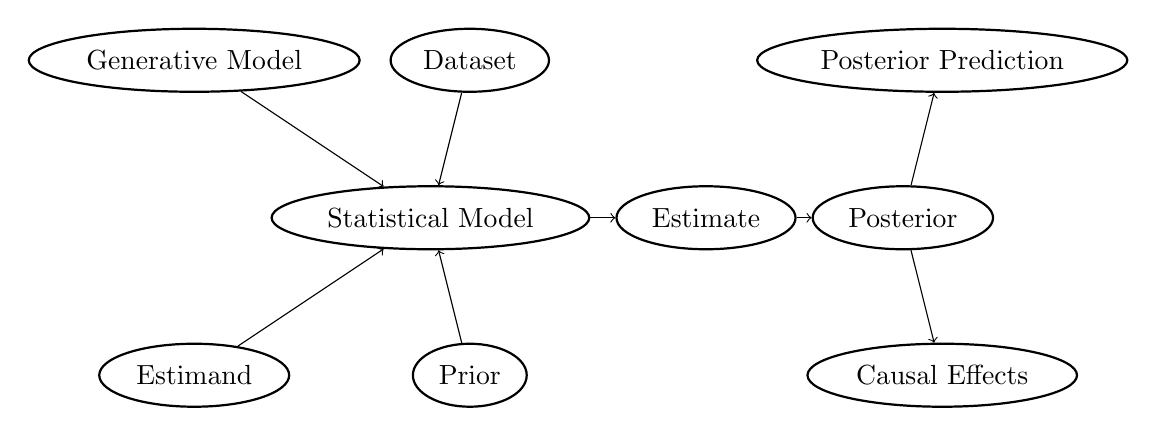
\begin{tikzpicture}[
    node distance=2cm,
    solid_node/.style={ellipse, draw, minimum size=8mm, thick},
    dashed_node/.style={ellipse, draw, dashed, minimum size=8mm, thick},
    directed/.style={-Stealth[scale=2], thick} 
]
        \node[solid_node] (G) at (0,4) {Generative Model};
        \node[solid_node] (Ed) at (0,0) {Estimand};
        \node[solid_node] (S) at (3,2) {Statistical Model};
        \node[solid_node] (Pi) at (3.5,0) {Prior};
        \node[solid_node] (D) at (3.5,4) {Dataset};
        \node[solid_node] (Et) at (6.5,2) {Estimate};
        \node[solid_node] (Po) at (9,2) {Posterior};
        \node[solid_node] (Pp) at (9.5,4) {Posterior Prediction};
        \node[solid_node] (CE) at (9.5,0) {Causal Effects};
    \draw [->] (G) -- (S);
    \draw [->] (Ed) -- (S);
    \draw [->] (Pi) -- (S);
    \draw [->] (D) -- (S);
    \draw [->] (S) -- (Et);
    \draw [->] (Et) -- (Po);
    \draw [->] (Po) -- (Pp);
    \draw [->] (Po) -- (CE);

    \end{tikzpicture}
    \caption{Core Bayesian Workflow, proposed in 305}
\end{figure}




\begin{figure}[h]
\centering 
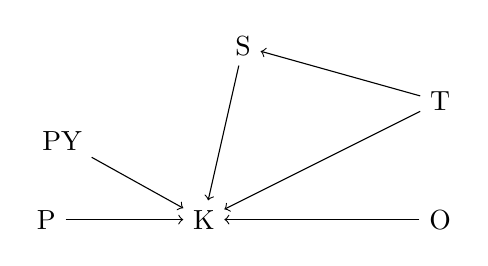
\begin{tikzpicture}[
    node distance=2cm,
    solid_node/.style={circle, draw, minimum size=8mm, thick},
    dashed_node/.style={circle, draw, dashed, minimum size=8mm, thick},
    directed/.style={-Stealth, thick} 
]
    \node (T) at (6,2.5) {T};
    \node (K) at (3,1) {K};
    \node (S) at (3.5,3.2) {S};
    \node (O) at (6,1) {O};
    \node (P) at (1,1) {P};
    \node (PY) at (1.2,2) {PY};
    \draw [->] (T) -- (S);
    \draw [->] (T) -- (K);
    \draw [->] (PY) -- (K);
    \draw [->] (S) -- (K);
    \draw [->] (P) -- (K);
    \draw [->] (O) -- (K);
\end{tikzpicture}
\caption{DAG of causalities among attributes of dataset - K: a ratio of Kouzu obsidians, S: a ratio of Shinshu obsidians, O: other sites, T: typology of artifacts or associated artifacts in the same layer, P: publication, PY: publication year.  }
\end{figure}


\begin{figure}[h]
\centering 
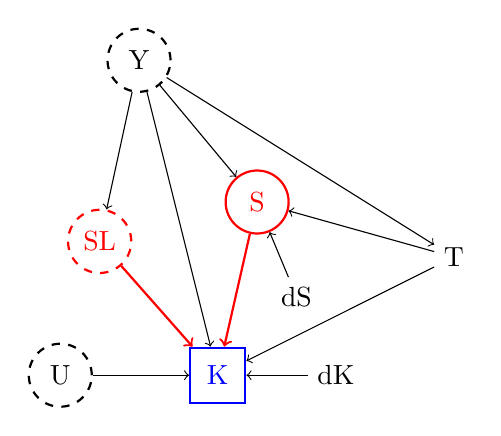
\begin{tikzpicture}[
    node distance=2cm,
    solid_node/.style={circle, draw, minimum size=8mm, thick},
    dashed_node/.style={circle, draw, dashed, minimum size=8mm, thick},
    directed/.style={-Stealth, thick} 
]
    \node[dashed_node] (Y) at (2,5) {Y};
    \node (T) at (6,2.5) {T};
    \node[dashed_node] (U) at (1,1) {U};
    \node[red, dashed_node] (SL) at (1.5,2.7) {SL};
    \node[blue, rectangle, draw, minimum size=7mm, thick] (K) at (3,1) {K};
    \node[red, solid_node] (S) at (3.5,3.2) {S};
    \node (dK) at (4.5,1) {dK};
    \node (dS) at (4,2) {dS};
    \draw [->] (Y) -- (T);
    \draw [->] (Y) -- (K);
    \draw [->] (Y) -- (S);
    \draw [->] (Y) -- (SL);
    \draw [->] (T) -- (S);
    \draw [->] (T) -- (K);
    \draw [->, red, thick] (SL) -- (K);
    \draw [->] (dS) -- (S);
    \draw [->] (dK) -- (K);
    \draw [->, red, thick] (S) -- (K);
    \draw [->] (U) -- (K);
\end{tikzpicture}
\caption{DAG of causalities among parameters - K: a ratio of Kouzu obsidians (blue solid square), S: a ratio of Shinshu obsidians (red dashed circle), SL: sea level difference based on current level (m; red dashed circle), T: typology of artifacts or associated artifacts in the same layer, dK: distance from Kozusima (km), dS: distance from the centre of Shinshu production sites (km), Y: true date (dashed circle as it is hidden), U: other hidden parameters influencing K (dashed). Colored arrows are from predictors to estimate. }
\end{figure}





\end{document}
